\documentclass[10pt, a4paper, twocolumn]{article}

\usepackage[slovak]{babel}
\usepackage[utf8]{inputenc}
\usepackage[text={18cm, 25cm}]{geometry}
\usepackage{fancyhdr}
\usepackage{times}
\usepackage{enumitem,kantlipsum}
\usepackage{graphics}
\usepackage{amsmath} 
\usepackage{amsthm}
\usepackage{float}

\setlength\parindent{0pt}
\pagestyle{fancy}

\lhead{Sabína Gregušová}
\chead{ISS Projekt 2018/2019}
\rhead{xgregu02}

\begin{document}

\section*{Vypracovaný protokol}
Tento projekt bol riešený v programe \texttt{GNU Octave} na základe znalostí nadobudnutých počas zimného semestra 2018/2019 v predmete Signály a systémy.

\begin{enumerate}[leftmargin=*]
%%% First task %%%
\item Použila som funkciu \texttt{audioread} na načítanie súboru \texttt{xgregu02.wav} a zistila som, že vzorkovacia frekvencia je 16~000 [Hz]. Súbor má teda 32~000 vzorkov za 2 sekundy.

%%% Second task %%%
\item Pomocou cyklu \texttt{for} som dekódovala každý ôsmy vzor zo segmentu 16-tich vzorkov a jeho odpovedajúcu hodnotu som si uložila do vektora \texttt{decoded}. Jeho obsah som si naformátovala do pomocného súboru a pomocou softvéru \texttt{Meld} som si overila, že môj spracovaný signál je identický so súborom zo zadania.

\begin{figure}[H]
\centering
\scalebox{0.40}{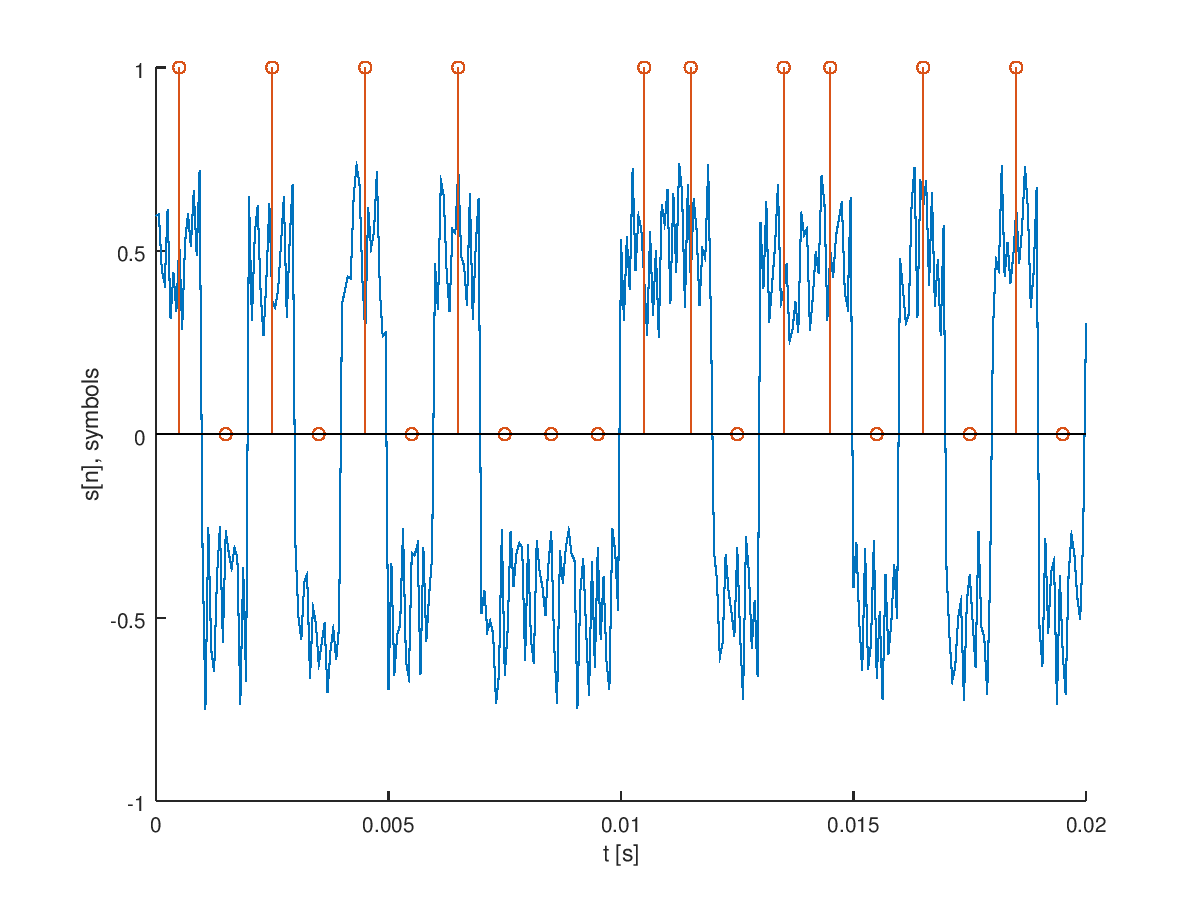
\includegraphics{second.png}}
\end{figure}

%%% Third task %%%
\item Aby bol filter stabilný, musia byť všetko jeho póly v jednotkovej kružnici, čiže musí platiť  $|p_k| < 1$ Pomocou funkcie \texttt{zplane} som vizualizovala túto skutočnosť na uvedenom obrázku a túto skutočnosť som skontrolovala pomocou funkcie \texttt{ukazmito}. Môžeme teda prehlásiť, že filter je stabilný.
\begin{figure}[H]
\centering
\scalebox{0.40}{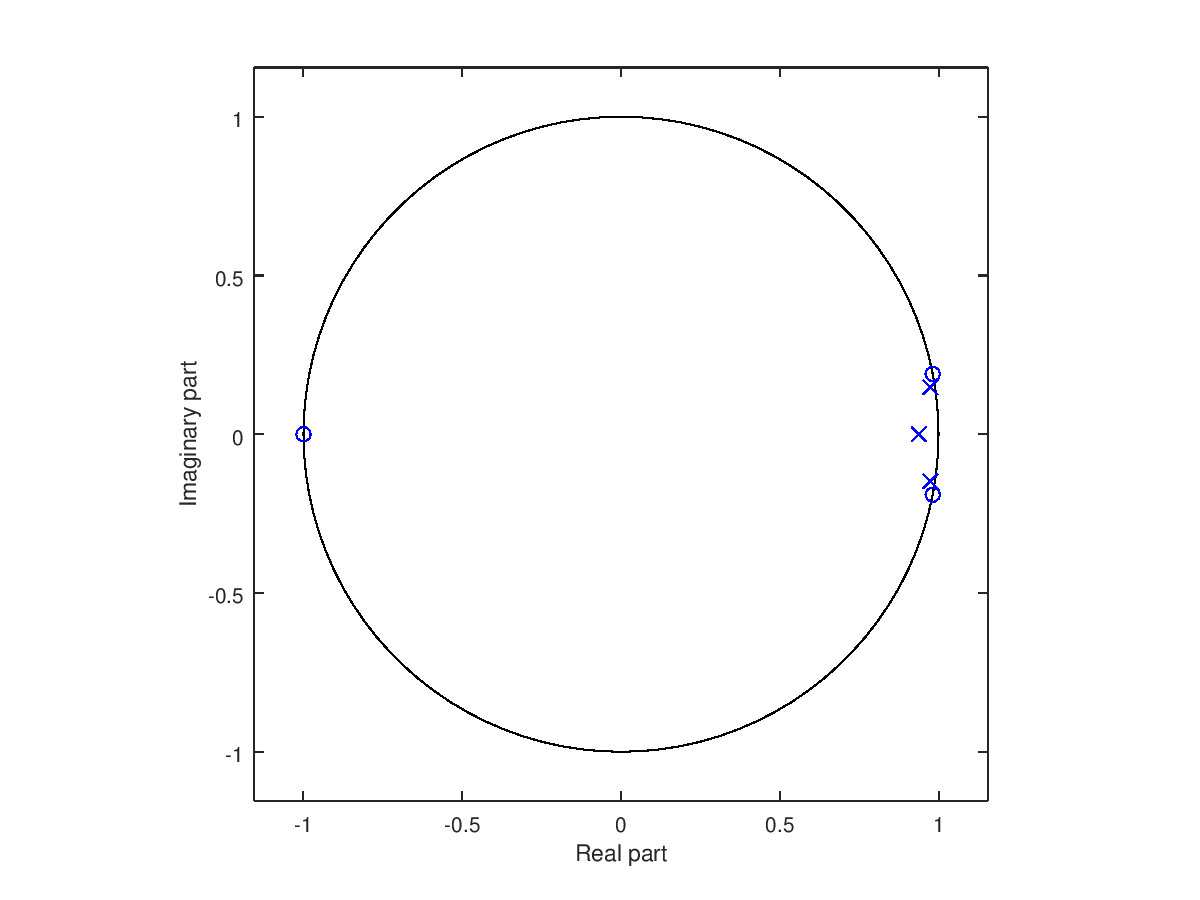
\includegraphics{stability.png}}
\end{figure}

%%% Fourth task %%%
\item Filter má dolnú propusť.
\begin{figure}[H]
\centering
\scalebox{0.40}{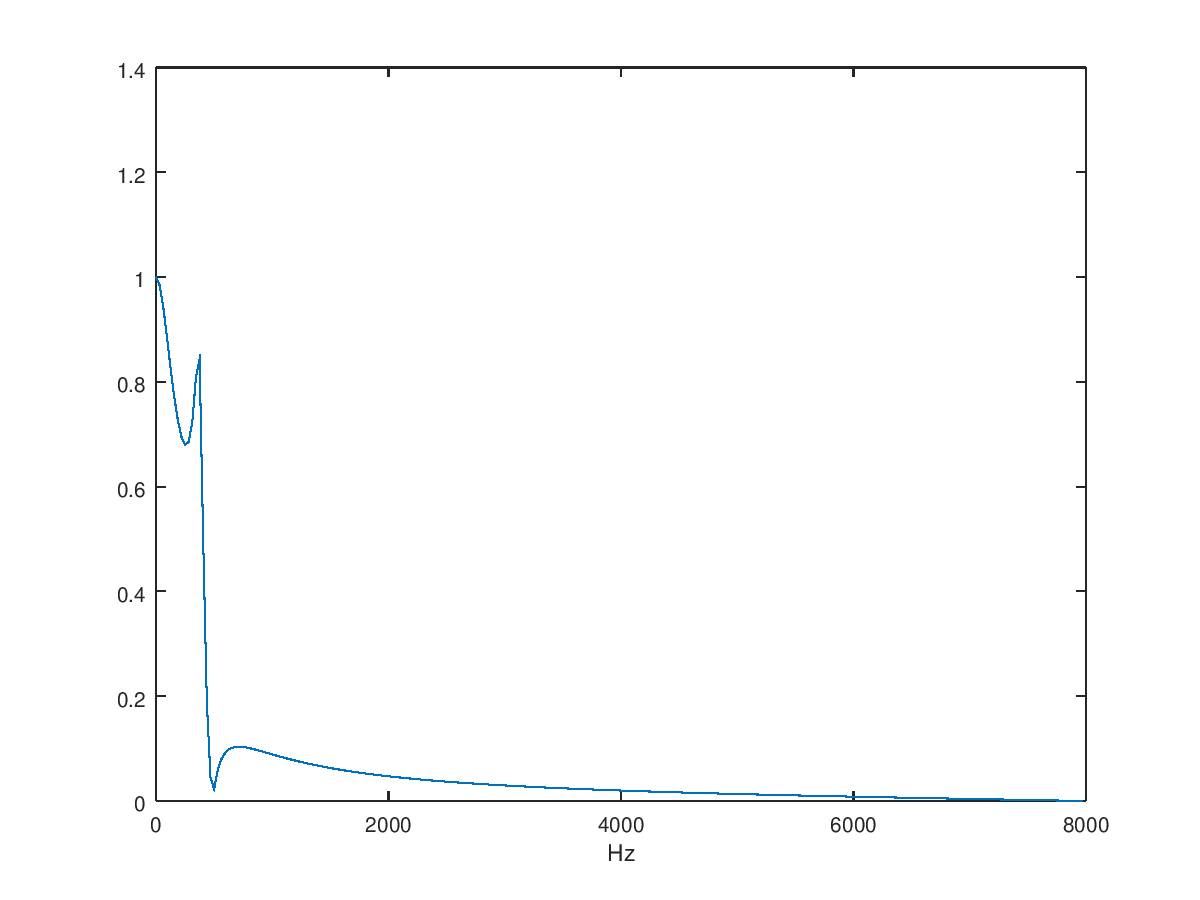
\includegraphics{charac.png}}
\end{figure}

%%% Fifth task %%%
\item Náš vstupný signál sme prefiltrovali filtrom a je na prvý pohľad je zrejmé, že nový signál $ss[n]$ je onsekorený.
\begin{figure}[H]
\centering
\scalebox{0.40}{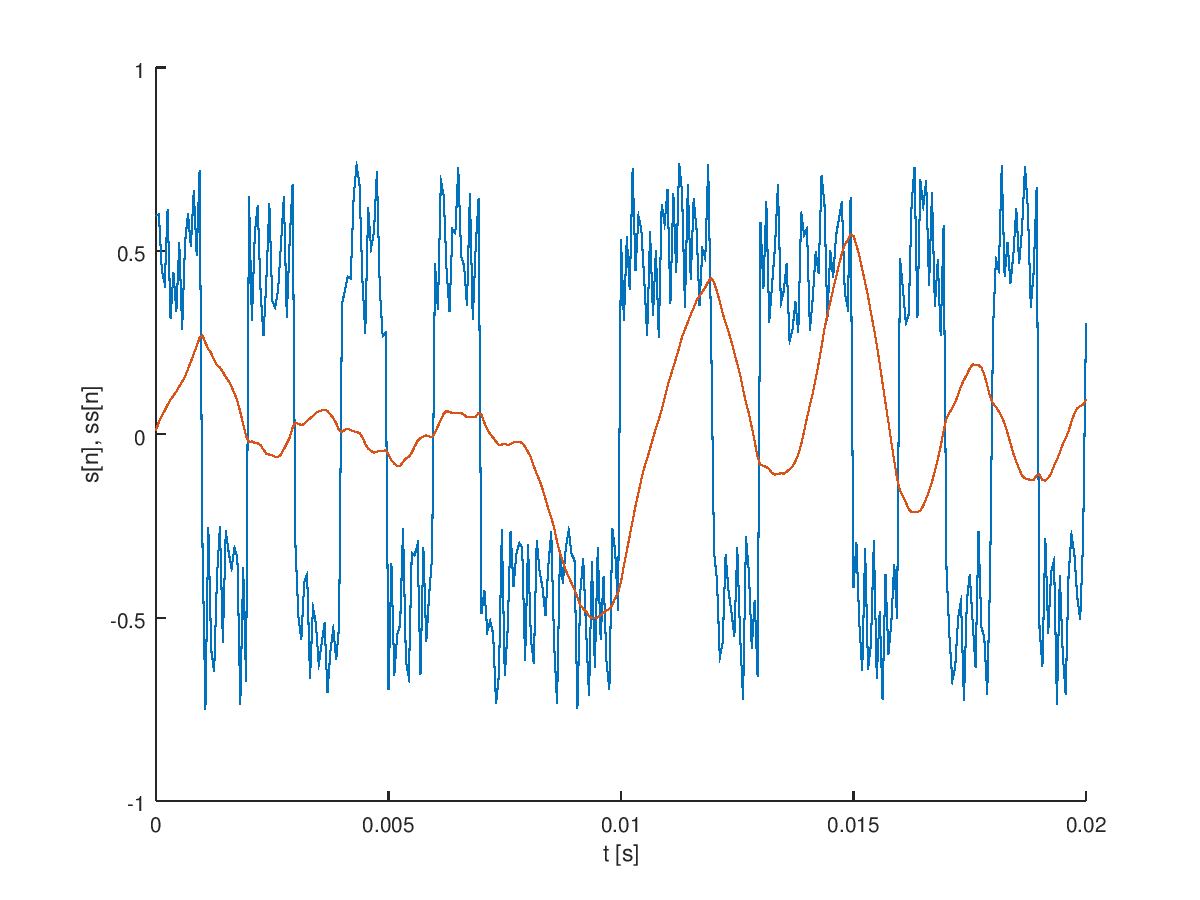
\includegraphics{filtered.png}}
\end{figure}

%%% Sixth task %%%
\item
\begin{figure}[H]
\centering
\scalebox{0.40}{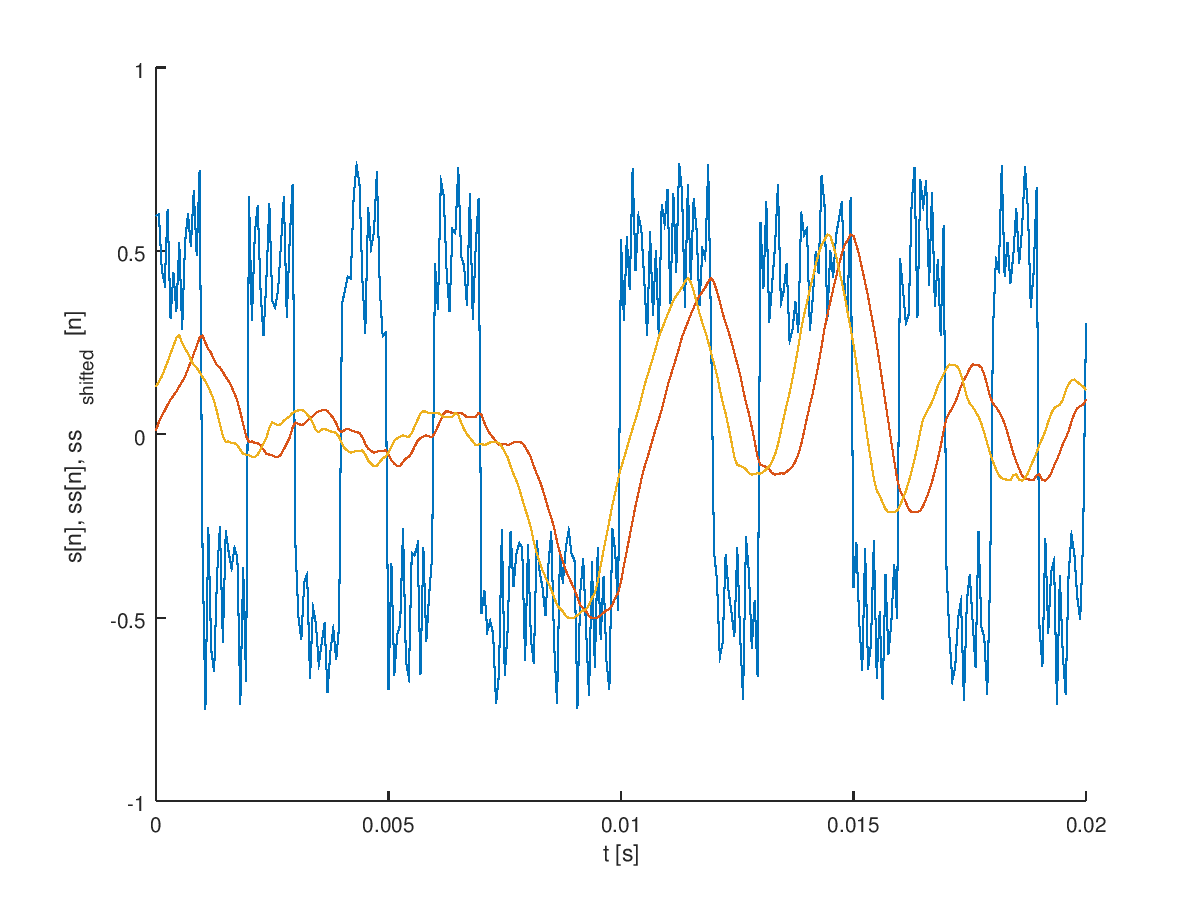
\includegraphics{shifted.png}}
\end{figure}

\item
\item
\item

%%% Tenth task %%%
\item Na výpočet autokorelačného koeficientu pomocou výrazu 
\begin{align}
R[k] = \frac{1}{N}\sum\limits_n x[n]x[n+k]\nonumber
\end{align}
 som použila funkciu \texttt{xcorr} s parametrom \texttt{biased}.
\begin{figure}[H]
\centering
\scalebox{0.40}{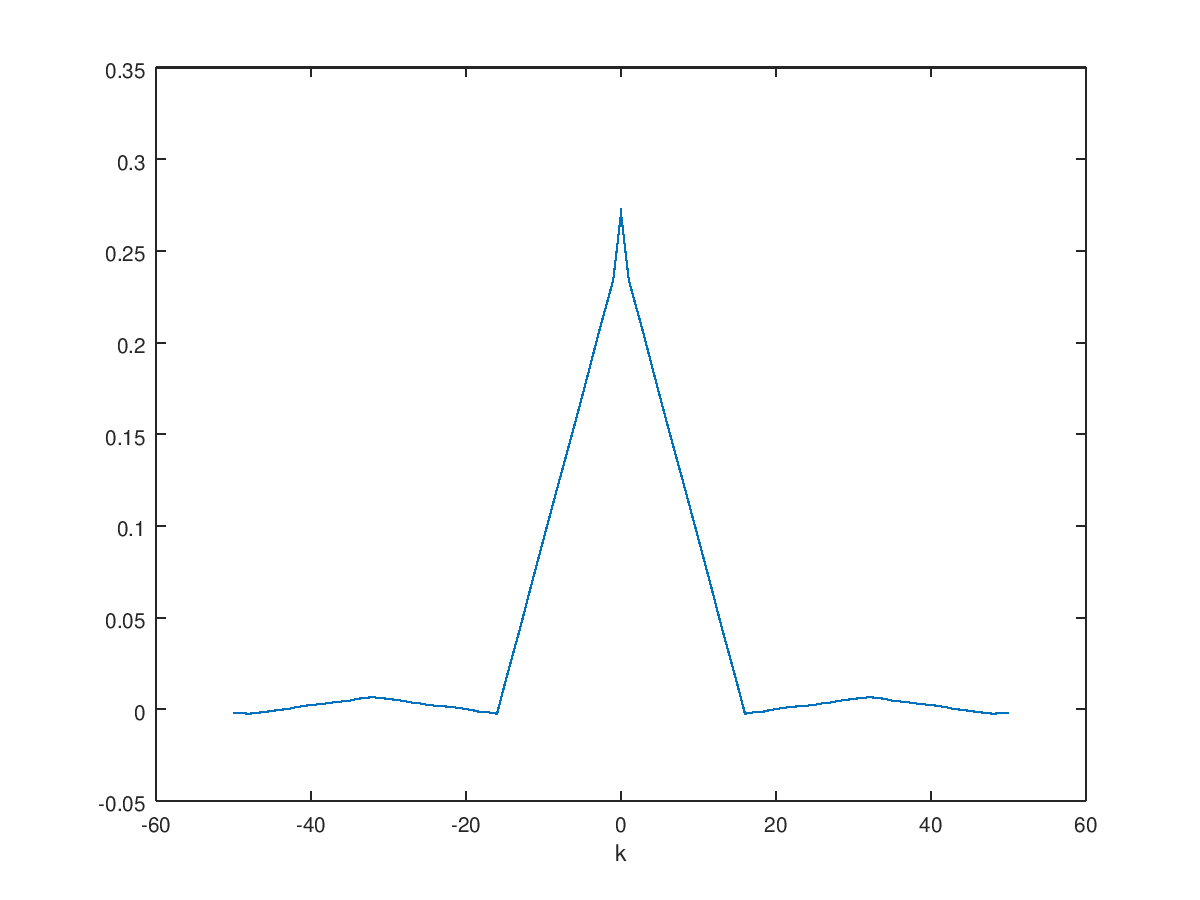
\includegraphics{corr.png}}
\end{figure}

%%% Eleventh task %%%
\item Museli sme uvažovať, že náš index je $k$, preto
\begin{align}
R[0] \quad&= 0.270576 \nonumber \\
R[1] \quad&= 0.234161 \nonumber \\
R[16] \quad&= -0.002462\nonumber
\end{align}

%%% Twelfth task %%%
\item Z funkcie v súbore \texttt{hist2opt.m} som si vybrala dôležité časti na výpočet  funkcie hustoty rozdelenia pradepodobnosti medzi vzorkami $n$ a $n+1$ a aplikovala som naň funkciu \texttt{imagesec}, ktorý vytvoril adekvátny obrázok. 
\begin{figure}[H]
\centering
\scalebox{0.40}{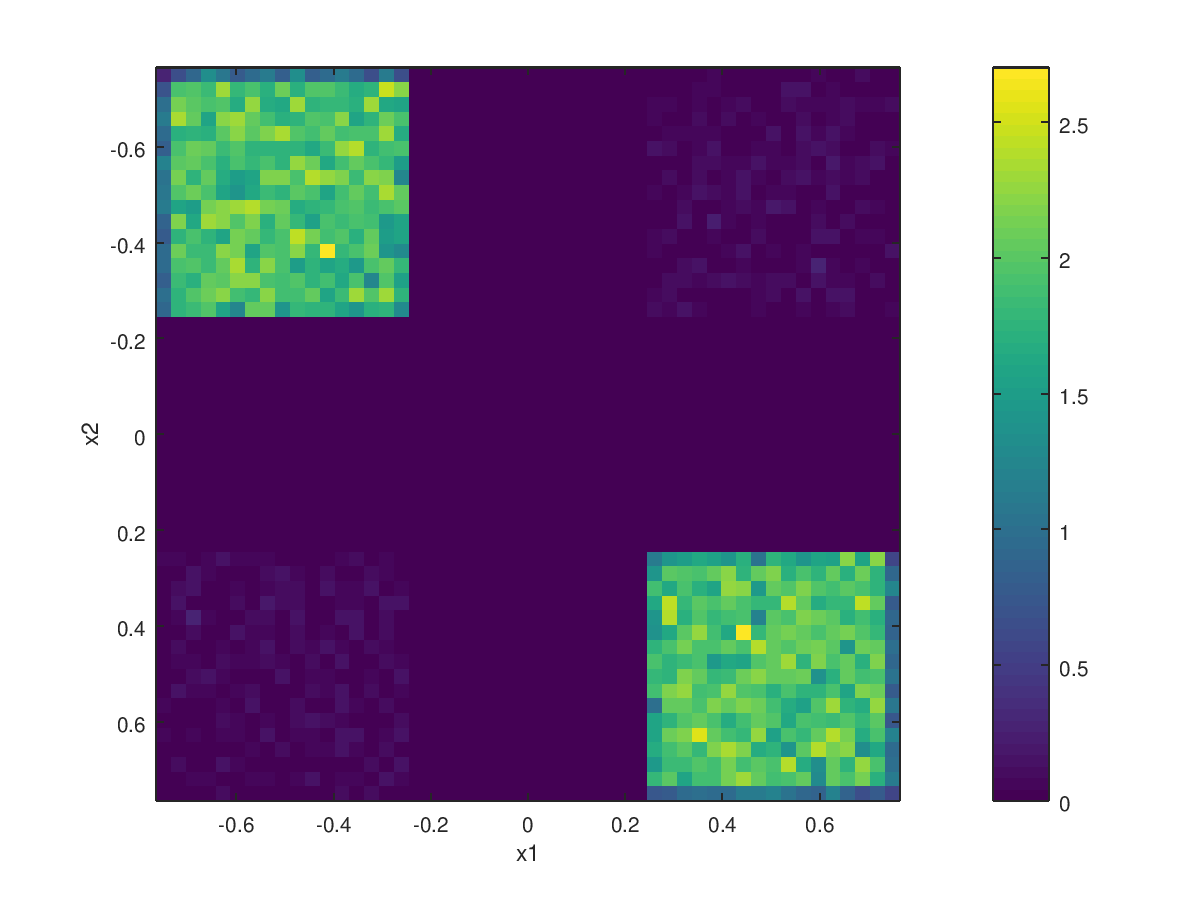
\includegraphics{distr.png}}
\end{figure}

%%% Thirtienth task %%%
\item Aby bola združená funkcia rozdelenia pravdepodobnosti správna, musí platiť:
\begin{align}
\int_{x_1} \int_{x_2} p(x_1, x_2, 1) dx_1 dx_2 = 1 \nonumber
\end{align}
Na základe príkazu \texttt{sum(sum(p))*surf} nám vyšla hodnota $0.99997$, čo môžeme považovať za správny výsledok s prihliadnutím na zaokrúhlovaciu chybu.

\item Výpočet som vykonala na základe funkcie zo súboru \texttt{hist2opt.m} a výsledok je
\begin{align}
R[1] = 0.234198 \nonumber
\end{align}
Ak porovnáme výsledok z úlohy č. 11, kde bol výsledok $R[1]=0.234161$, môžeme prehlásiť, že sú zhodné a rozdiel je spôsobený len chybou zaokrúhľovania a preto je teda zanedbateľná.

\end{enumerate}

\end{document}